% !TeX root = ../../../main.tex

The possibility of an intrinsic charm component was recently studied
in~\cite{Hou:2017khm}, by modifying the CT14 \pdf set, with the
initial 4\fns charm \pdf taken equal to the BHPS
model~\cite{Brodsky:1980pb} form with the normalization fitted as a
free parameter.
%
A 4\fns  charm \pdf with uncertainties at $Q=1.3$~GeV was then
constructed by taking 
the BHPS model with best-fit normalization as central value (called
the `BHPS1 model' in~\cite{Hou:2017khm}); the lower
edge of the uncertainty band was taken to coincide with the standard
CT14 charm \pdf  (i.e.\ the charm \pdf determined by perturbative
matching from the 3\fns to the 4\fns); the upper edge of the uncertainty
band was taken as 
the BHPS model but with  normalization fixed to the upper  90\% CL limit (called the
`BHPS2 model' in~\cite{Hou:2017khm}).

%%%%%%%%%%%%%%%%%%%%%%%%%%%%%%%%%%%%%%%%%%%%%%%%%%%%%%%%%%%%%%%%%%%
\begin{figure}[h]
  \begin{center}
    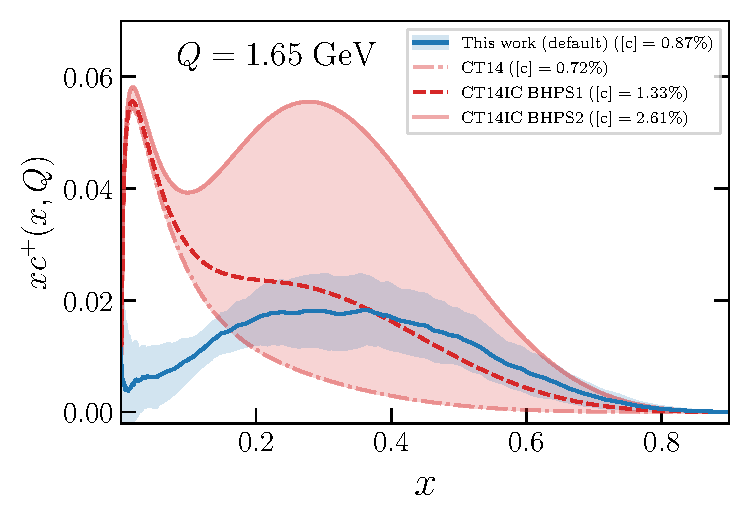
\includegraphics[width=0.49\linewidth]{ch-ic/pdfplot-abs-lin-charm-q1p65gev.pdf}
    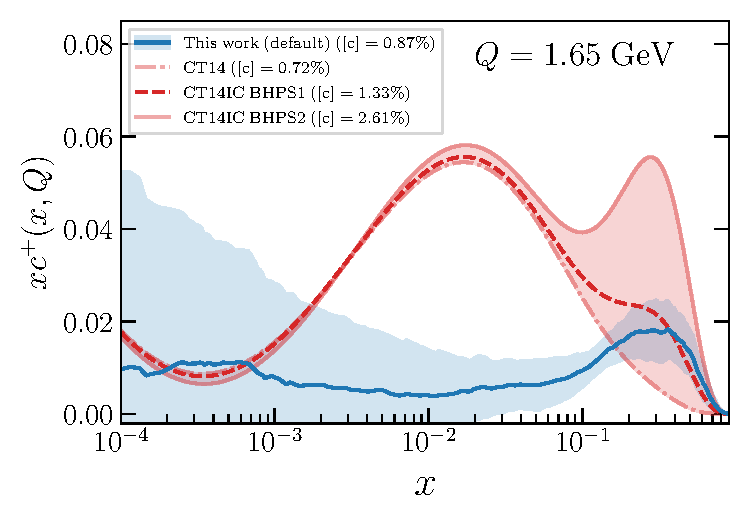
\includegraphics[width=0.49\linewidth]{ch-ic/pdfplot-abscharm-q1p65gev.pdf}
    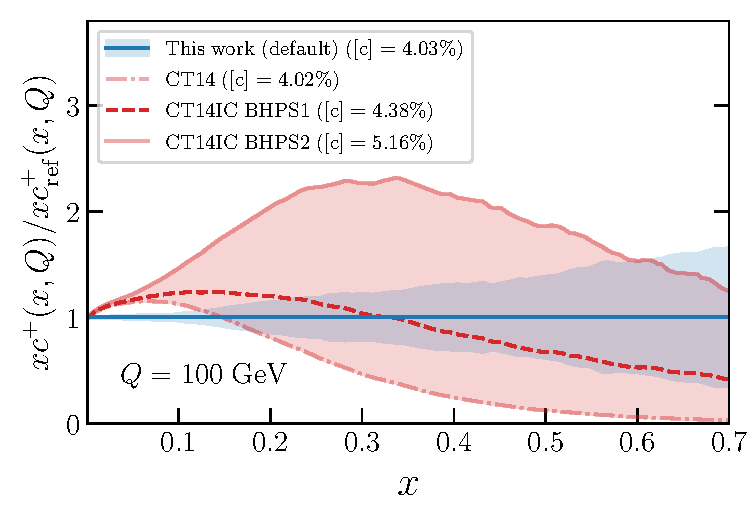
\includegraphics[width=0.49\linewidth]{ch-ic/pdfplot-abscharm-q100gev.pdf}	
    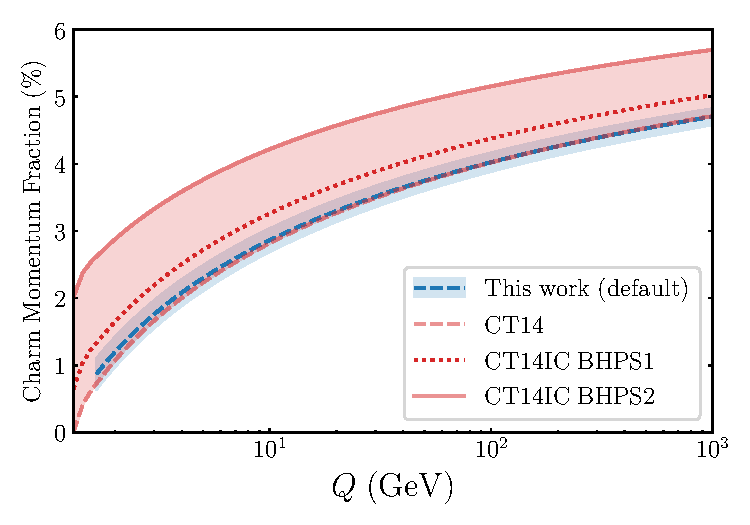
\includegraphics[width=0.49\linewidth]{ch-ic/charm_momfrac_qdep_ct.pdf}
    \caption{\small The 4\fns charm \pdf
    from~\cite{Hou:2017khm} compared to our result (also in the 4\fns) 
     at $Q=1.65$~GeV on
    a linear (top left) and logarithmic (top right) scale in $x$, and
    at  $Q=100$~GeV on a linear scale in $x$ and as a ratio to our result
    (bottom left).
    %
    The momentum fraction corresponding to either case
    is also shown as a function of $Q$ (bottom right). Note that for
    our result the uncertainty band is the 68\%CL \pdf uncertainty,
    while for~\cite{Hou:2017khm} the central curve (labeled
    CT14IC BHPS1) corresponds to the BHPS model with best-fit
    normalization, the lower curve (labeled
    CT14) corresponds to the default CT14 perturbative charm \pdf and
    the upper curve (labeled
    CT14IC BHPS2) corresponds to the BHPS model with normalization at
    the upper 90\% CL (see text). The value of the momentum fractions
    are also provided in each case.
  \label{fig:ic/comparison_CT14} }
\end{center}
\end{figure}
%%%%%%%%%%%%%%%%%%%%%%%%%%%%%%%%%%%%%%%%%%%%%%%%%%%%%%%%%%%%%%%%%%%%%%

The CT14IC charm \pdf is compared to our result in
Fig.~\ref{fig:ic/comparison_CT14}, at  $Q=1.65$ GeV and $Q=100$ GeV, in
the former case on both a logarithmic and linear scale in $x$ and in
the latter case on a linear scale only, as a ratio to our default
result.
%
Note that the uncertainty band has a different interpretation in the
two curves shown: for our result it is the 68\%~CL \pdf uncertainty,
while for~\cite{Hou:2017khm}  it corresponds to the model
uncertainty estimated as described above.
%
In Fig.~\ref{fig:ic/comparison_CT14} we also quote
the charm momentum fraction in each case, at the corresponding scale $Q$. 

As shown in Fig.~\ref{fig:ic/charm_content_3fns} (right), our result for
the charm \pdf is in good agreement with the BHPS model at large
$x$. Correspondingly, for $x\gsim 0.3$
we find reasonably good agreement between our
result and the central curve of~\cite{Hou:2017khm}, which
corresponds to a momentum fraction and thus a normalization of the charm
\pdf not too different from our result (see Table~\ref{tab:ic/momfrac_lowQ}).
%
Both the upper and lower curve from~\cite{Hou:2017khm} instead
do not agree with our result within uncertainties: indeed the
lower edge corresponds to the absence of intrinsic charm (which we
exclude) and the upper edge to a momentum fraction which we exclude
at more than the $5\sigma$ level (see Table~\ref{tab:ic/momfrac_lowQ}). 

For intermediate values $3\cdot10^{-3}\lsim x\lsim 0.3$  our result disagrees
with that of 
~\cite{Hou:2017khm}, while at very small $x$ all results agree,
the intrinsic charm being compatible with zero.
The disagreement at intermediate $x$ is mostly due
to the fact that in ~\cite{Hou:2017khm} charm is assumed to take
the BHPS form, which vanishes for $x\lsim 0.1$,
in the 4\fns at the low scale $Q=1.3$~GeV.
%
Due to perturbative evolution from  $Q=1.3$~GeV to $Q=1.65$~GeV the charm 
\pdf then develops the large bump that is
seen in Fig.~\ref{fig:ic/comparison_CT14}, where we instead find that 
the 4\fns charm \pdf is quite small.
%
This difference persists at large scales as seen  in
Fig.~\ref{fig:ic/charm_content_3fns} (bottom left).

In terms of momentum fractions, shown in Fig.~\ref{fig:ic/charm_content_3fns} (bottom right),
as already mentioned our result is
compatible with the central value of~\cite{Hou:2017khm} within
uncertainties; and also with the lower edge of ~\cite{Hou:2017khm}
that corresponds to perturbative charm.
%
The upper edge  of the prediction from~\cite{Hou:2017khm} is instead
ruled out at more than $5\sigma$. 
